%-----------------------------------
% Define document and include general packages
%-----------------------------------
\documentclass[12pt,oneside,titlepage,listof=totoc,bibliography=totoc]{scrartcl}
\usepackage[utf8]{inputenc}
\usepackage[ngerman]{babel}
\usepackage[babel,german=quotes]{csquotes}
\usepackage[T1]{fontenc}
\usepackage{fancyhdr}
\usepackage{fancybox}
\usepackage[a4paper, left=4cm, right=2cm, top=2.8cm, bottom=2.3cm]{geometry}
\usepackage{graphicx}
\usepackage{colortbl}
\usepackage{array}
\usepackage{float}      %Positionierung von Abb. und Tabellen mit [H] erzwingen
\usepackage{footnote}
\usepackage{caption}
\usepackage{mdwlist}
\usepackage{amssymb}
\usepackage{mathptmx}
\usepackage{amsmath}
\usepackage[table]{xcolor}
\usepackage{marvosym}			% Verwendung von Symbolen, z.B. perfektes Eurozeichen
\usepackage[colorlinks=true,linkcolor=black]{hyperref}
\definecolor{darkblack}{rgb}{0,0,0}
\hypersetup{colorlinks=true, breaklinks=true, linkcolor=darkblack, menucolor=darkblack, urlcolor=darkblack}
\usepackage{times}
\fontfamily{ptm}\selectfont

% Mehrere Fussnoten nacheinander mit Komma separiert
\usepackage[multiple]{footmisc}
% todo Aufgaben als Kommentare verfassen für verschiedene Editoren
\usepackage{todonotes}

%Pakete für Tabellen
\usepackage{epstopdf}
\usepackage{nicefrac} % Brüche
\usepackage{multirow}
\usepackage{rotating} % vertikal schreiben
\usepackage{colortbl}
\usepackage{mdwlist}

\definecolor{dunkelgrau}{rgb}{0.8,0.8,0.8}
\definecolor{hellgrau}{rgb}{0.0,0.7,0.99}
% Colors for listings
\definecolor{mauve}{rgb}{0.58,0,0.82}
\definecolor{dkgreen}{rgb}{0,0.6,0}

% sauber formatierter Quelltext
\usepackage{listings}
\lstset{numbers=left,
	numberstyle=\tiny,
	numbersep=5pt,
	breaklines=true,
	showstringspaces=false,
	frame=l ,
	xleftmargin=5pt,
	xrightmargin=5pt,
	basicstyle=\ttfamily\scriptsize,
	stepnumber=1,
	keywordstyle=\color{blue},          % keyword style
  	commentstyle=\color{dkgreen},       % comment style
  	stringstyle=\color{mauve}         % string literal style
}

% Biblatex
\usepackage[
backend=biber,
style=numeric,
citestyle=authoryear,
bibstyle=verbose,
url=false,
isbn=false,
notetype=footonly,
hyperref=false,
sortlocale=de]{biblatex}

%weitere Anpassungen für BibLaTex
% Optionen für Biblatex
\ExecuteBibliographyOptions{%
  giveninits=false,
  isbn=true,
  url=true,
  doi=false,
  eprint=false,
  maxbibnames=7,      % Alle Autoren (kein et al.)
  maxcitenames=2,     % et al. ab dem 3. Autor
  backref=false,      % Rückverweise auf Zitatseiten
  bibencoding=utf8,   % wenn .bib in utf8, sonst ascii
  bibwarn=true        % Warnung bei fehlerhafter bib-Datei
}%

% et al. an Stelle von u.a.
\DefineBibliographyStrings{ngerman}{
   andothers = {{et\,al\adddot}},                   % TODO et.al. prüfen
}

% Klammern um das Jahr in der Fußnote
\renewbibmacro*{cite:labelyear+extrayear}{%
  \iffieldundef{labelyear}                          % TODO footcite anpassen
    {}
    {\printtext[bibhyperref]{%
       \mkbibparens{%
         \printfield{labelyear}%
         \printfield{extrayear}}}}}

\DeclareNameFormat{last-first}{%
  \iffirstinits
    {\usebibmacro{name:family-given}
        {\namepartfamily}
        {\namepartgiveni}
        {\namepartprefix}
        {\namepartsuffix}
    }
    {\usebibmacro{name:family-given}
        {\namepartfamily}
        {\namepartgiven}
        {\namepartprefix}
        {\namepartsuffix}
    }%
  \usebibmacro{name:andothers}}


% Alternative Notation der Fußnoten
% Zeigt sowohl den Nachnamen als auch den Vornamen an
% Beispiel: \fullfootcite[Vgl. ][Seite 5]{Tanenbaum.2003}
\DeclareCiteCommand{\fullfootcite}[\mkbibfootnote]    % TODO Autor nur Inital als Vornamen!
  {\printtext{Vgl.\isdot}}                            % TODO Bsp.-PDF anpassen
  {\usebibmacro{citeindex}%                           % TODO Zahlen [] raus
    \addspace\textit{\printnames[sortname][1-1]{author}}%
    \addcomma\addspace\printfield{shorttitle}\addcomma\space
    \addspace\printfield{year}\addcomma\space
  }
  {\printtext{S.\isdot}\space}
  {\printfield{pages}}

%Autoren (Nachname, Vorname)
\DeclareNameAlias{default}{family-given}
%\DeclareNameAlias{sortname}{family-given}

%Reihenfolge von publisher, year, address verändern
% Achtung, bisher nur für den Typ @book definiert

%% Definiert @Book Eintrag         % TODO pages f. ff.
\DeclareBibliographyDriver{book}{%
  \textit{\printnames{author}}%
  \newunit\space
  \printtext{$($}%
  \printfield{shorttitle}%         % TODO durch Stichwort ersetzen
  \setunit*{\addcomma\space}%
  \printfield{year}%
  \printtext{$)$}%
  \setunit*{\addcolon\space}%
  \printfield{title}%
  \setunit*{\addcomma\space}%
  \printfield{edition}%
  \setunit*{\addcomma\space}%
  \printlist{location}%           % TODO falls mehr als drei Orte u.a.
  \setunit*{\addcolon\space}%
  \printlist{publisher}%
  \setunit*{\addcomma\space}%
  \printfield{year}%
  %\newunit\newblockpunct
}

%% Definiert @Online Eintrag    % TODO Overhaule needed
\DeclareBibliographyDriver{online}{%
  \printnames{author}%
  \newunit\newblockpunct
  \printfield{title}%
  \setunit*{,\space}%
  %\newunit\newblock
  \printfield{url}%
  \setunit*{,\space Erscheinungsjahr:\space}%
  \printfield{year}%
  \setunit*{,\space Aufruf am:\space}%
  \printfield{note}%
}
  
%% Definiert @Article Eintrag
\DeclareBibliographyDriver{article}{%
  \printnames{author}%
  \newunit\newblockpunct
  \printfield{title}%
  \setunit*{.\space In:\space}%
  %\newunit\newblock
  \usebibmacro{journal}%
  \setunit*{\space (}%
  \printfield{year}\newunit{)}%
}

%Doppelpunkt nach dem letzten Autor
%\renewcommand*{\labelnamepunct}{\addcolon\addspace}

%Komma an Stelle des Punktes, nach Autor
%\renewcommand*{\newunitpunct}{\addcomma\space}

%Leerzeichen an Stelle des Punktes, nach Autor
\renewcommand*{\newunitpunct}{\space}

%Autoren durch Semikolon trennen
%\newcommand*{\bibmultinamedelim}{\addsemicolon\space}%
%\newcommand*{\bibfinalnamedelim}{\addsemicolon\space}%
%\AtBeginBibliography{%
%  \let\multinamedelim\bibmultinamedelim
%  \let\finalnamedelim\bibfinalnamedelim
%}

%Titel nicht kursiv anzeigen 
\DeclareFieldFormat{title}{#1\isdot}
%\finentry % dot


%Bib-Datei einbinden
\addbibresource{literatur/literatur.bib}

% Pfad fuer Abbildungen
\graphicspath{{./}{./abbildungen/}}

%-----------------------------------
% Weitere Ebene einfügen
\usepackage{titletoc}

\makeatletter

% Setze die Tiefe des Inhaltsverzeichnis auf 4 Ebenen%
% Damit erscheinen \paragraph-Sektionen auch im Inhaltsverzeichnis
\setcounter{secnumdepth}{4}
\setcounter{tocdepth}{4}

% Fuege Abstand nach unten wie in einer normalen \section hinzu
% Andernfalls haette \paragraph keinen Zeilenumbruch
% Der Zeilenumbruch koennte mit einer leeren \mbox{} ersetzt werden
% Jedoch klebt dann der Text relativ nah an der Ueberschrift
\renewcommand{\paragraph}{%
  \@startsection{paragraph}{4}%
  {\z@}{3.25ex \@plus 1ex \@minus .2ex}{1.5ex plus 0.2ex}%
  {\normalfont\normalsize\bfseries\rmfamily}%
}
% TODO Abstand über Titel
\makeatother


%-----------------------------------
% Zeilenabstand 1,5-zeilig
%-----------------------------------
\usepackage{setspace}
\onehalfspacing

%-----------------------------------
% Absätze durch eine neue Zeile
%-----------------------------------
\setlength{\parindent}{0mm}
\setlength{\parskip}{0.8em plus 0.5em minus 0.3em}

\sloppy					%Abstände variieren
\pagestyle{headings}

%-----------------------------------
% Abkürzungsverzeichnis
%-----------------------------------
\usepackage[intoc]{nomencl}
\renewcommand{\nomname}{Abkürzungsverzeichnis}
\setlength{\nomlabelwidth}{.20\textwidth}
\renewcommand{\nomlabel}[1]{#1 \dotfill}
\setlength{\nomitemsep}{-\parsep}
\makenomenclature

%-----------------------------------
% Meta informationen
%-----------------------------------
%-----------------------------------
% Meta Informationen zur Arbeit
%-----------------------------------

% Autor
\newcommand{\myAutor}{Thomas Eiling}

% Adresse
\newcommand{\myAdresse}{Eichsfelder Weg 4b \\ \> \> 46359 Heiden}

% Titel der Arbeit
\newcommand{\myTitel}{Testautomatisierung von PHP-Projekten dargestellt an einem Shopware Projekt}

% Betreuer
\newcommand{\myBetreuer}{Dipl.-Kfm. Henning Mertes}

% Lehrveranstaltung
\newcommand{\myLehrveranstaltung}{Modul Nr. 1}

% Matrikelnummer
\newcommand{\myMatrikelNr}{313489}

% Ort
\newcommand{\myOrt}{Duisburg}

% Datum der Abgabe
\newcommand{\myAbgabeDatum}{10. Dezember 2016}

% Semesterzahl
\newcommand{\mySemesterZahl}{7}

% Name der Hochschule
\newcommand{\myHochschulName}{FOM Hochschule für Oekonomie \& Management Essen}

% Standort der Hochschule
\newcommand{\myHochschulStandort}{Standort Duisburg}

% Studiengang
\newcommand{\myStudiengang}{Wirtschaftsinformatik}

% Art der Arbeit
\newcommand{\myThesisArt}{Bachelor Thesis}

% Zu erlangender akademische Grad
\newcommand{\myAkademischerGrad}{Bachelor of Science (B. Sc.)}

% Firma
\newcommand{\myFirma}{Mustermann GmbH}

%-----------------------------------
% Kopfbereich / Header definieren
%-----------------------------------
\pagestyle{fancy}
\fancyhf{}
\fancyhead[R]{\thepage}								% Seitenzahl oben, rechts
%\fancyhead[L]{\leftmark}							% kein Footer vorhanden
\renewcommand{\headrulewidth}{0.4pt}


%-----------------------------------
% Start the document here:
%-----------------------------------
\begin{document}

\pagenumbering{Roman}								% Seitennumerierung auf römisch umstellen
\renewcommand{\refname}{Literaturverzeichnis}		% "Literatur" in
%"Literaturverzeichnis" umbenennen
\newcolumntype{C}{>{\centering\arraybackslash}X}	% Neuer Tabellen-Spalten-Typ:
%Zentriert und umbrechbar

%-----------------------------------
% Titlepage
%-----------------------------------
\begin{titlepage}
	\newgeometry{left=2cm, right=2cm, top=2cm, bottom=2cm}
	\begin{center}
		\textbf{\myHochschulName}\\
		\textbf{\myHochschulStandort}\\
		\vspace{1.5cm}
			
\includegraphics[width=3cm]{abbildungen/fomLogo.jpg} \\
		\vspace{1.5cm}
		Berufsbegleitender Studiengang\\
		\myStudiengang, \mySemesterZahl. Semester\\
		\vspace{2cm}
		\textbf{\myThesisArt}\\
		\textbf{zur Erlangung des Grades eines}\\
		\textbf{\myAkademischerGrad}\\
		% Oder für Hausarbeiten:
		%\textbf{im Rahmen der Lehrveranstaltung}\\
		%\textbf{\myLehrveranstaltung}\\
		\vspace{2cm}
		über das Thema\\
		\Huge{\myTitel}\\
		\vspace{0.2cm}
	\end{center}
	\normalsize
	\vfill
	\begin{tabbing}
		Links \= Mitte \= Rechts\kill
		Betreuer: \> \> \myBetreuer\\
		\> \> \\

		Autor: \> \> \myAutor\\
		\> \>  Matrikelnr.: \myMatrikelNr\\
		\> \> \myAdresse\\
		\> \> \\
		Abgabe: \> \> \myAbgabeDatum
	\end{tabbing}
\end{titlepage}

%-------Ende Titelseite-------------

%-----------------------------------
% Sperrvermerk
%-----------------------------------
%\newpage
\thispagestyle{empty}

%-----------------------------------
% Sperrvermerk
%-----------------------------------
\section*{Sperrvermerk}
Die vorliegende Abschlussarbeit mit dem Titel \enquote{\myTitel} enthält unternehmensinterne Daten der Firma \myFirma . Daher ist sie nur zur Vorlage bei der FOM sowie den Begutachtern der Arbeit bestimmt. Für die Öffentlichkeit und dritte Personen darf sie nicht zugänglich sein.

\vspace{5cm}

\begin{table}[H]
	\centering
	\begin{tabular*}{\textwidth}{c @{\extracolsep{\fill}} ccccc}
		\myOrt, \today
		&
		% Hinterlege deine eingescannte Unterschrift im Verzeichnis /abbildungen und nenne sie unterschrift.png
		% Bilder mit transparentem Hintergrund können teils zu Problemen führen
		\includegraphics[width=0.35\textwidth]{unterschrift}\vspace*{-0.35cm}
		\\
		\rule[0.5ex]{12em}{0.55pt} & \rule[0.5ex]{12em}{0.55pt} \\
		(Ort, Datum) & (Eigenhändige Unterschrift)
		\\
	\end{tabular*} \\
\end{table}

\newpage


%-----------------------------------
% Inhaltsverzeichnis
%-----------------------------------
\setcounter{page}{1}
\tableofcontents
\newpage

%-----------------------------------
% Abkürzungsverzeichnis
%-----------------------------------
\printnomenclature
\newpage
%-----------------------------------
% Abbildungsverzeichnis
%-----------------------------------
\listoffigures
\newpage
%-----------------------------------
% Tabellenverzeichnis
%-----------------------------------
\listoftables
\newpage
%-----------------------------------
% Seitennummerierung auf arabisch und ab 1 beginnend umstellen
%-----------------------------------
\pagenumbering{arabic}
\setcounter{page}{1}
%-----------------------------------
% Kapitel / Inhalte
%-----------------------------------
\section{Einleitung}
Der Bereich der IT-Security hat in den letzten Jahren zunehmend an Bedeutung gewonnen, was vor allem auf die steigenden Fallzahlen von Cyberkriminalität zurückzuführen ist. Insbesondere Vorfälle großer Datenverluste bei namhaften Unternehmen rücken das Thema in den medialen Fokus und schaffen ein wachsendes Bewusstsein für die Bedeutung der Cybersicherheit. Dies hat eine steigende Nachfrage nach effektiven Lösungen zur Sicherung digitaler Infrastrukturen und deren Überwachung zur Folge.

Im Kontext der Überwachung von Netzwerken entstehen bereits in kleinen Infrastrukturen riesige Datenmengen, die von Menschen nicht in akzeptabler Zeit ausgewertet werden können. Diese Herausforderung führt dazu, dass wertvolle Informationen nicht aktiv zur Verbesserung der Netzwerksicherheit genutzt werden können. Eine vielversprechende Lösung zur Bewältigung dieses Problems ist der Einsatz von \ac{SOAR}-Systemen. Diese Systeme unterstützen Sicherheitsteams dabei, Sicherheitsereignisse effektiv zu orchestrieren und automatisieren.

\ac{SOAR}-Systeme ermöglichen \cite{PICUS.2023} die kontinuierliche Überwachung von Netzwerken und sind mittlerweile ein integraler Bestandteil von Security Operation Centern. Sie aggregieren Ereignisse aus verschiedenen Quellen und stellen diese in Echtzeit dar, was die Effizienz der Sicherheitsoperationen erheblich steigert und eine Automatisierung ermöglicht. Angesichts der kritischen Rolle, die solche Systeme in der IT-Infrastruktur von Unternehmen spielen, ist eine fehlerfreie Funktionsweise unerlässlich. Zudem müssen \ac{SOAR}-Systeme robust gegenüber Angriffen sein und eine geringe Fehleranfälligkeit aufweisen, um den Anforderungen an moderne Sicherheitsarchitekturen gerecht zu werden.

\begin{comment}
\subsection{Zielsetzung}
Kleiner Reminder für mich in Bezug auf die Dinge, die wir bei der Thesis beachten sollten und \LaTeX{}-Vorlage für die Thesis.

\subsection{Aufbau der Arbeit}
Kapitel \ref{infos} enthält die Inhalte des Thesis-Days und alles, was zum inhaltlichen erstellen der Thesis relevant sein könnte. In Kapitel \ref{latexDetails} \nameref{latexDetails} findet ihr wichtige Anmerkungen zu \LaTeX{}, wobei die wirklich wichtigen Dinge im Quelltext dieses Dokumentes stehen (siehe auch die Verzeichnisstruktur in Abbildung \ref{fig:verzeichnisStruktur}).


\begin{figure}[H]
\caption{Verzeichnisstruktur der \LaTeX{}-Datein}\label{fig:verzeichnisStruktur}

\includegraphics[width=0.9\textwidth]{verzeichnisStruktur}
\\
Quelle: Eigene Darstellung
\end{figure}
\end{comment}
\newpage
\section{Grundlagen der Auswertung unstrukturierter Daten} \label{infos}
Siehe auch Wissenschaftliches Arbeiten~\footcite[\vglf][S. 1]{savic.2020}. %ohne textcommands
Damit sollten alle wichtigen Informationen abgedeckt sein ;-)~\footcite[\vglf][\pagef 1]{savic.2020} %mit textcommands
Hier gibt es noch ein Beispiel für ein direktes Zitat\footcite[][\pagef 1]{savic.2020} %mit textcommands

\subsection{Text Preprocessing} \label{TextPreprocessing}
Text Mining bezeichnet den Prozess, um wesentliche bekannte aber auch unbekannte Informationen aus Textdaten zu
generieren~\footcite[\vglf][\pagef 1]{mohan.2015}
Die Verarbeitung von unstrukturierten Textdaten wird auch als \ac{KDT}
bezeichnet und spielt eine signifikate Rolle in Anwendungsgebieten wie

\begin{itemize}
    \item Information Retrieval
    \item Information Extraction
    \item Natural Language Processing~\footcite[\vglf][\pagef 1 f.]{mohan.2015}
\end{itemize}
Im Wesentlichen geht es in allen \og Anwendungsgebieten um die Wissen durch das Mining der Texte zu generieren.

\begin{figure}[H]
    \caption{Text Mining Prozess}\label{fig:2_1_1_KDT_Process}
    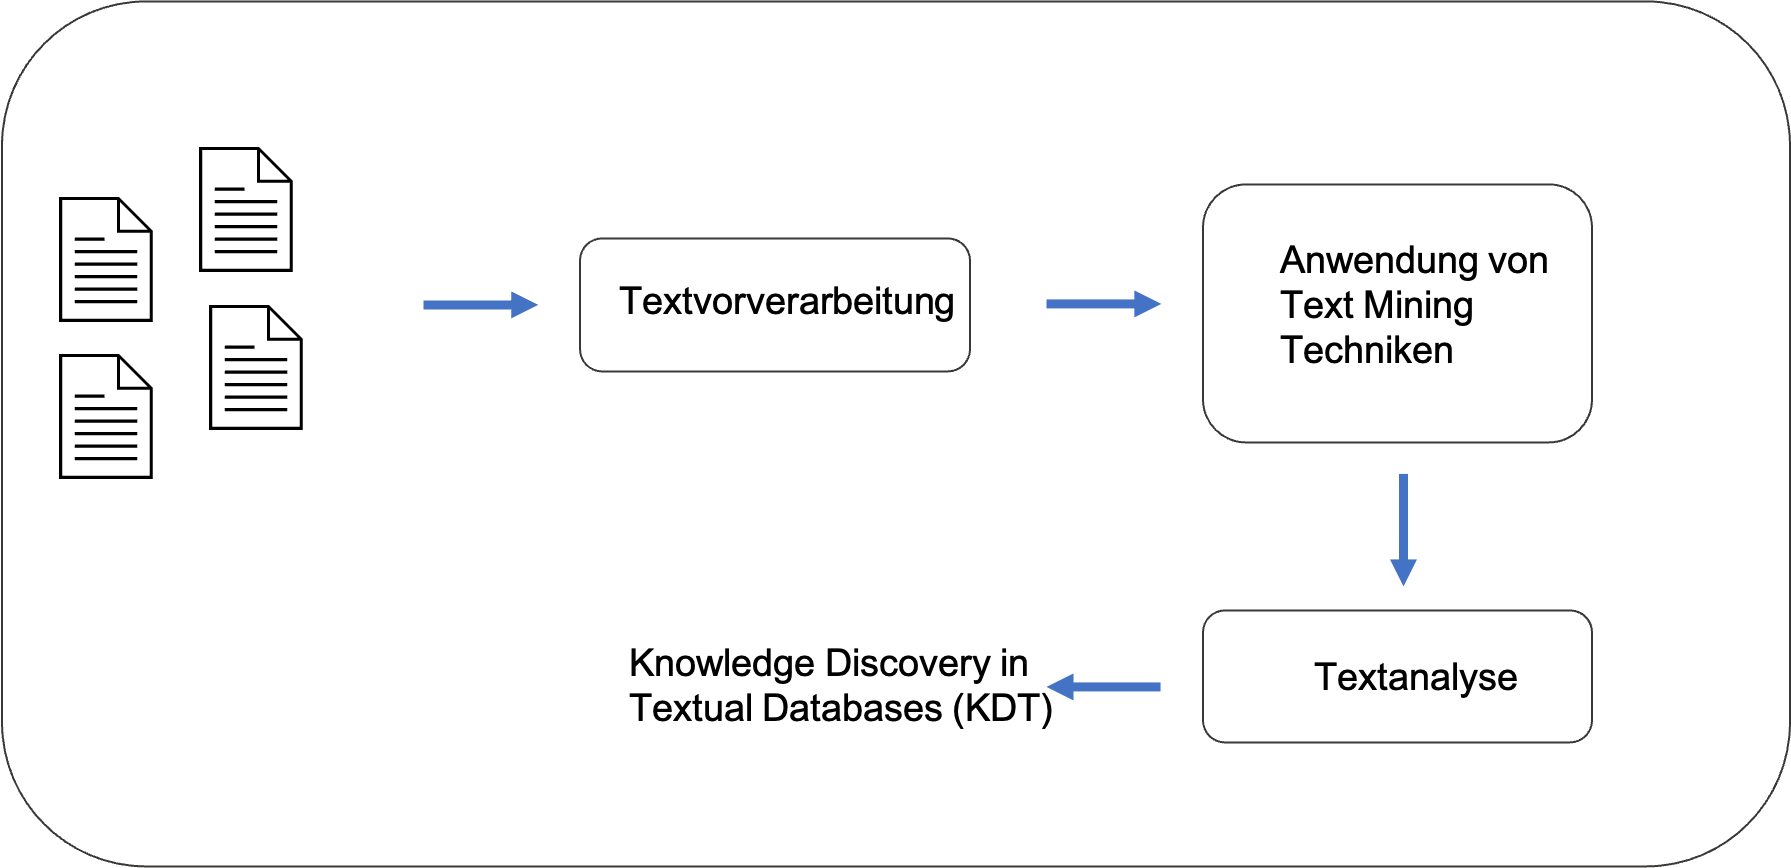
\includegraphics[width=0.9\textwidth]{2_1_1_KDT_Process}
    \\
    \textit{Quelle: Eigene Darstellung in Anlehnung an}~\cite[\pagef 1]{mohan.2015}
\end{figure}

Wie der Abbildung{}\ref{fig:2_1_1_KDT_Process} entnommen werden kann, stellt die Vorverarbeitung von Volltextdaten bei nahe
zu jeder Aufgabe im \ac{NLP} einen essentiellen und kritischen Schritt dar,
da hierbei die fundamentale Basis für die Weiterverarbeitung
sowie die Entwicklung der Modelle geschaffen wird.~\footcite[\vglf][\pagef 2]{gurusamy.2014}
Der Begriff der Textvorverarbeitung umfasst dabei die Anwendung unterschiedlicher Techniken/Methoden, bei
denen die Textdokumente für die eigentlichen Zielsetzungen vorbereitet werden.
Gängige Techniken für die Vorbereitung der Texte für die nachgelagerten Analysen können folgendermaßen aufgeteilt
werden:~\footcite[\vglf][\pagef 1]{pahwa.2018}

\begin{itemize}
    \item Inhalte Extrahieren und Bereinigen
    \item Annotationen
    \item Normalisieren
\end{itemize}

Zu Beginn der Volltextanalysen stehen häufig die Rohfassungen der Texte zur Verfügung.
Diese gilt es im ersten Schritt technisch einzulesen.
Hierbei werden auch Daten mit eingelesen, dessen Informationsgehalt gering ist.
Beispielshaft zu nennen sind hier HTML tags, Werbung, etc beim Auslesen einer Website~\footcite[\vglf][\pagef 1]
{pahwa.2018} oder Grafiken, ASCII-Codes in PDF-Dateien.
Demnach ist das Ziel bei dem \textbf{Extrahieren und Bereinigen
der Inhalte} die Rohdaten soweit zu säubern, bis sich schließlich die reinen Texte als Resultat ergeben.
Nachdem die Texte um die technischen Störfaktoren bereinigt wurden, ist die \textbf{Tokenization} eine typische Technik
der Textextraktion.
In dem Prozess der Tokenisation wird der gesamte zu analysierende Text in einzelne Wörter, Phrasen,
Symbole, etc.
geteilt.
Hierbei wird das Ziel verfolgt die Bedeutung einzelner Wörter innerhalb eines Satzes zu analysieren.
Die Tokens dienen nämlich als Eingabewerte für viele weitergehende Prozessschritte.~\footcite[\vglf][\pagef 2]
{gurusamy.2014}
In jedem Text befinden sich Wörter, die wenig Informationsgehalt bei der Textanalyse bieten.
Solche Wörter werden auch als \textbf{Stop Words} bezeichnet.
Beispiele für solche Stop Words sind Artikel oder
Präpositionen wie \glqq{der}\grqq, \glqq{die}\grqq, \glqq{das}\grqq, \glqq{ein}\grqq,
\glqq{in}\grqq, \glqq{mit}\grqq, etc.
Im Analyseprozess stellt jedes unterschiedliche Wort eine eigene Dimension dar.
Durch die Entfernung der Stop Words wird somit die Dimensionshöhe reduziert bei gleichzeitiger Beibehaltung des
Informationsgehaltes des jeweiligen Satzes/Textes.~\footcite[\vglf][\pagef 3]{mohan.2015}\\
Neben der klassischen Methode, die Stop Words auf Basis einer vordefinierten Liste zu entfernen, sind diverse
mathematische und nicht-mathematische Methoden entwickelt worden, um Stop Words in Texten zu identifizieren und zu
bereinigen.\footnote{Detailiertere Informationen zu unterschiedlichen Methoden für die Entfernung von Stop Words
können{}\cite{mohan.2015} entnommen werden.}\\

\textcolor{red}{Annotationen: POS ergänzen!!!!}
Die Annotationen eines Textes sollen die Funktion des jeweiligen Wortes im Kontext des gesamten Satzes identifizieren.
\\


Bei dem \textbf{Normalisieren} von Texten wird das Ziel verfolgt ähnliche Wörter zu vereinheitlichen bzw.
diese auf einen Standard zu bringen.
Dieser Prozess soll vor allem die Dimensionen reduzieren, um die Berechnungen zu vereinfachen und gleichzeitig die
Effizienz durch die Standardiesierung der Wörter erhöhen.
\newline
Bei der Normalisierung von Wörtern wird häufig auf die Techniken des \textbf{Stemming} oder der \textbf{Lemmatization}
zurückgegriffen.
Das Stemming ist ein Prozess, der zugrundeliegende Wörter auf den Wortstamm herunterbricht.~\footcite[\vglf][\pagef 5]
{khyani.2021}
Dieser Wortstamm ist im Ergebnis häufig kein echtes Wort, sondern oftmals eine Buchstabenkombination bzw.
ein Präfix, den viele Wörter gemeinsam haben.~\footcite[\vglf][\pagef 5]{khyani.2021}
Es existiert eine Vielzahl an Stemming-Algorithmen, dessen Performance vom jeweiligen Einsatzbereich abhängt, sodass
noch kein Standard etabliert ist.\footnote{Eine ausführliche Analyse unterschiedlicher Stemming-Algorithmen kann{}
\cite{jivani.2011} entnommen werden.}
\newline
Die Idee bei der Lemmatization ist das so genannte \grqq{Lemma}\grqq{} oder auch die Vokabularform eines Wortes
zu identifizieren.~\footcite[\vglf][\pagef 7]{khyani.2021}
Der Prozess ist ähnlich dem des Stemmings, jedoch mit dem Unterschied im Ausgabewert.
Während beim Stemming der Ausgabewert der Wortstamm ist und oftmals kein echtes Wort,
ist der Ausgabewert bei der Lemmatization das Grundwort aus beispielsweise einem Wörterbuch.~\footcite[\vglf]
[\pagef 7]{khyani.2021}
Die Abbilung{}\ref{fig:2_1_2_Stem_Lemma} verdeutlicht die Unterschiede der Lemmatization und des Stemmings anhand
des englischen Wortes \grqq{change}\grqq{} bzw.
dessen Abwandlungen.

\begin{figure}[H]
    \caption{Stemming vs. Lemmatization}\label{fig:2_1_2_Stem_Lemma}
    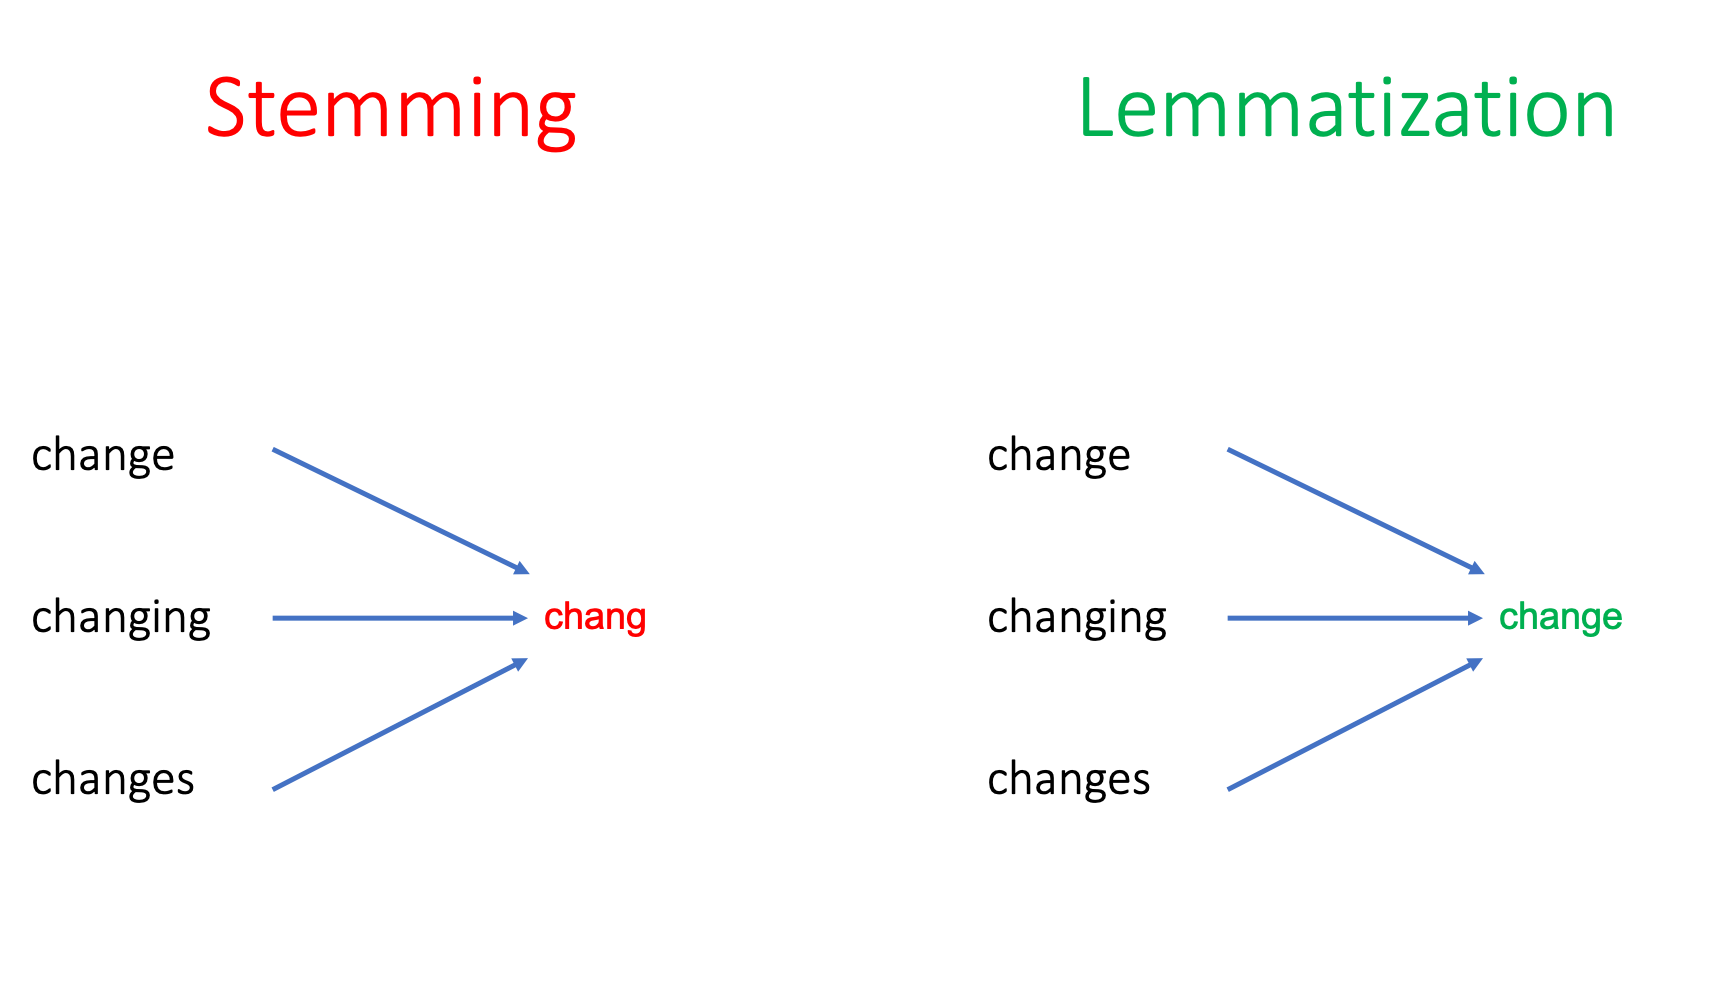
\includegraphics[width=0.9\textwidth]{2_1_2_Stem_Lemma}
    \\
    \textit{Quelle: Eigene Darstellung in Anlehnung an}~\cite[\pagef 7]{khyani.2021}
\end{figure}
Ein vorab durchgeführtes \ac{POS}-Tagging kann die Ergebnisse der Lemmatization optimieren.
Wenn das Wort \glqq{schloss}\grqq{} nämlich in einem Text als Nomen durch das \ac{POS}-Tagging erkannt wird,
dann handelt es sich dabei je nach Kontext entweder um ein Schloss zum verriegeln oder um ein Schloss als Gebäude.
Wird es dagegen als Verb identifiziert, so wird mit einer hohen Wahrscheinlichkeit zum Lemma \glqq{schließen}\qrqq{}
umgewandelt.

\subsection{Named Entity Recognition} \label{NER}

\begin{itemize}
    \item Was ist NER
    \item Wie kommen wir an Daten und Tools?
    \item Was sind NER-Möglichkeiten - Klassische NER / DL-NER)
\end{itemize}
Mithilfe der \ac{NER} wird das Ziel verfolgt automatisiert Eigennamen in Texten zu identifizieren,
dessen semantische Typen wie beispielsweise Personen, Ort, Organisationen vordefiniert wurden.~\footcite[\vglf]
[\pagef 1]{nadeau.2007}
Die \ac{NER} kann nicht nur ausschließlich für die Extraktion von Informationen aus Texten genutzt werden, viel mehr
spielt sie eine wesentliche Rolle in einer Vielzahl von Anwendungen aus dem Gebiet des \ac{NLP} wie beispielsweise dem
Textverständnis, dem \ac{IR}, automatisierter Textzusammenfassungen und Übersetzungen, Fragenbeantwortungen, etc.
In der Forschung existiert eine Vielzahl an Definitionen für die zu erkennenden Eigennamen, die hauptsächlich in
folgende zwei Kategorien aufgeteilt werden können:
\begin{itemize}
    \item Generische (\zb Personen und Ort)
    \item Domänenspezifische (\zb Proteine, Enzyme und Gene)~\footcite[\vglf][\pagef 1]{li.2020}
\end{itemize}
Bei den in der \ac{NER} angewandten Techniken wird zwischen
\begin{itemize}
    \item Regelbasierte Ansätze
    \item Unüberwachte Ansätze
    \item Merkmalsbasierte überwachte Lernansätze
    \item Deep-Learning Ansätze
\end{itemize}
unterschieden, wobei die drei erstgenannten den traditionellen Ansätzen zugehörig sind.~\footcite[\vglf][\pagef 1]
{li.2020}
Regelbasierte Systeme beruhen auf manuell erstellten Regeln.
Die zugrundeliegenden Regeln können hierbei \zb aus domänenspezifischen Ortsverzeichnisen oder syntaktisch-lexikalischen
Mustern abgeleitet worden sein.\newline
Das Clustering ist ein typischer Ansatz für unüberwachte \ac{NER}-Systeme.~\footcite[\vglf][\pagef 6 f.]{nadeau.2007}
Auf Basis von Kontextähnlichkeiten werden geclusterte Gruppen generiert aus denen schiließlich die
Entitäten extrahiert werden.
Die Idee bei dieser Technik ist mithilfe eines großen Corpus lexikalische Muster und Statistiken zu berechnen, um daraus
auf im Text benannte Entitäten schließen zu können.~\footcite[\vglf][\pagef 4]{li.2020}\newline
Im Teilbereich der überwachten Ansätze ist \ac{NER} hauptsächlich eine Klassifikationsaufgabe.
Ausgehend von annotierten Datensätzen werden Merkmale entwickelt, um jedes Trainingsbeispiel zu repräsentieren.
~\footcite[\vglf][\pagef 4]{li.2020}
Für die Entwicklung der Modelle kommen dann Algorithmen des \ac{ML} zu Einsatz, um aus den gegeben annotierten
Datensätzen Vorhersagemodelle für noch ungesehene Daten zu erlernen.~\footcite[\vglf][\pagef 4]{li.2020}
Essentiell in überwachten \ac{NER}-Systemen ist die Entwicklung der Merkmale.
Merkmalsvektoren abstrahieren dabei den Text, bei der ein Wort durch einen oder mehrere boolische, numerische oder
nominale Werte dargestellt wird.~\footcite[\vglf][\pagef 7]{nadeau.2007}\newline
Neben den eben erläuterten traditionellen Methoden für die \ac{NER} wurden in den letzten Jahren Ansätze im Bereich des
\ac{DL} entwickelt, welche sich bewährt haben und Spitzenergebnisse erzielen.~\footcite[\vglf][\pagef 5]{li.2020}
Der Einsatz von \ac{DL} hat wesentliche Vorteile gegenüber den traditionellen Methoden.
Zum einen ist es durch die besondere Architektur und den Verarbeitungsmöglichkeiten im Bereich des \ac{DL} über
mehrschichtige künstliche neuronale Netze möglich nicht-lineare Zusammenhänge zu erkennen und zu lernen und zum anderen
erleichtern \ac{DL}-basierte Modelle durch ihre Automation und Selbstständigkeit beim Lernen die Arbeit.~\footcite
[\vglf][\pagef 5]{li.2020}\newline
\newline
Die \ac{NER} umfasst zwei Teilaufgaben: Typenidentifikation und Grenzerkennung
Die Bewertung eines entwickelten \ac{NER}-Systems wird in der Regel durch den Vergleich mit den mennschlich getätigten
Annotationen vorgenommen.
Der Vergleich kann entweder über eine exakte oder durch eine partielle Übereinstimmungsevaluation vorgnommen werden.
~\footcite[\vglf][\pagef 3 f.]{li.2020}
Bei der exakten Übereinstimmungsevaluation wird geprüft, ob das System sowohl den richtigen Typen als auch die Grenzen
korrekt identifiziert.~\footcite[\vglf][\pagef 3]{tjongkimsang.2003}
Bei der partiellen Übereinstimmungsevaluation genügt es, wenn, unabhängig von den Grenzen, eine korrekte Identifikation
des Typen vom System vorgenommen wird, solange es eine Überschneidung zwischen den ermittelten Grenzen und den wahren
Grenzen gibt.
Bewertungskennzahlen für die Qualität des \ac{NER}-Systems sind Precision, Recall und der F-Score.
Um diese zu ermitteln, wird vorab die Anzahl der \ac{FP}, \ac{FN} und \ac{TP} Zuordnungen ermittelt.
\begin{itemize}
    \item \ac{FP}: Eine Entität wurde vom System erkannt, welche in Wirklichkeit keine ist
    \item \ac{FN}: Eine Entität wurde nicht vom System erkannt, welche in Wirklichkeit jedoch eine darstellt
    \item \ac{TP}: Eine Entität wurde vom System korrekt erkannt
\end{itemize}

Die Precision stellt sich dar als
\begin{align}
    Precision {=} \frac{\ac{TP}}{(\ac{TP}+{\ac{FP}})}
\end{align}
und kann als Verhältnis von richtig erkannten Entitäten zur Gesamtheit an identifizierten Entitäten interpretiert werden.

Der Recall
\begin{flalign}
    Recall{} {=} {}\frac{\ac{TP}}{(\ac{TP}+{\ac{FN}})}
\end{flalign}
bezieht die richtig erkannten Entitäten auf die Gesamtheit aller möglich gewesenen Entitäten.

Der ausgeglichene F-Score vereint die Precision und den Recall zu einem harmonischen Mittel:
\begin{flalign}
    F-Score{} {=} {}2 \cdot \frac{Precision \cdot Recall}{Precision + Recall}
\end{flalign}


\subsection{Named Entity Linking} \label{NEL}
\newpage
\section{Praxis} \label{sec:Praxis}
\subsection{Erstellung eines domänenspezifischen NER Modells}\label{sec:ErstellungNerModell}
Wie im Kapitel \ref{sec:NER} erläutert, lässt sich zwischen allgemeinen und domänenspezifischen \ac{NER}-Modellen unterscheiden.\footcite[vgl.][S.47]{nouvel2016} Domänenspezifische Modelle sind dabei solche, die für einen dedizierten Themenbereich erstellt wurden und daher in diesem Kontext besonders gute Ergebnisse erzielen.
Es gibt bereits spezialisierte Modelle im Bereich der Medizin die mit einem medizinischen Korpus trainiert wurden. Dazu zählen zum Beispiel BioBERT, ScispaCy oder Y\footcite[S.12]{li2020}. Diese beinhalten bereits zahlreiche medizinische Konzepte und Entitäten, allerdings mussten wir feststellen, dass auch sie für unseren Anwendungsfall \textit{out of the box} nicht alle erforderlichen Entitäten der hier betrachteten Domäne erkennen. Daher haben wir uns entschlossen ein eigenes Modell für das Themengebiet der Urtikaria-Forschung auf Basis eines sciSpacy Modells zu erstellen.
\subsubsection{Labeling von Trainingsdaten}\label{sec:Labeling}
Das Annotieren von Trainingsdaten hat einen zentralen Anteil bei der Erstellung eines eigenen Modells. Akkurate Daten sind essentiell für die Genauigkeit des resultierenden Modells. Neben der Menge der zum Training zur Verfügung stehenden Daten ist es unterlässlich, dass diese widerspruchsfrei sind.

\subsubsection{Auswahl der Labels}\label{sec:AuswahlLabels}
Die Auswahl der Labels muss für den Anwendungsfall angemessen sein. Je nachdem was die Zielstellung des Projektes ist, können unterschiedliche Labels erforderlich sein, um die notwendigen Zusammenhänge abzubilden.
In der vorliegenden Arbeit wurden 5 Entitäten ausgewählt. Diese sind Disease, Treatment, Biomarker, Diagnostic und Person. Die hier getroffene Auswahl basiert zum einen auf in der einschlägigen Literatur gewählten Labels und zum anderem auf den im Rahmen des CAPTUM Projektes umrissenen Entitäten.\footcite[vgl.][S.]{li2016}\footcite[vgl.][S.]{eickhoff2020}

% \subsubsection{Annotierungsaufgaben}

\subsubsection{Richtlinien zur Annotation}\label{sec:Richtlinien}
Um möglichst homogene, gleichmäßige Annotationen über mehrere Personen hinweg zu erhalten ist es sinnvoll Richtlinien für die Annotation festzulegen. Dies ist häufig ein iterativer Prozess, da zu Beginn einer solchen Aufgabe nicht immer vorab klar ist, an welchen Stellen Unklarheit besteht.[Citation]

Auch wir haben Richtlinien aufgestellt, die sich zum einen mit den von uns gewählten Entitäten selber und zum anderen mit der Art und Weise der Annotation beschäftigen. Die begrifflichen Definitionen sind vor allem vor dem Hintergrund wichtig, dass die beteiligten Personen keinen medizinischen Hintergrund haben und auf diese Art und Weise zunächst ein gemeinsames Grundverständnis davon geschaffen werden soll, was zum Beispiel einen \textit{Biomarker} oder \textit{Diagnostik} ausmacht. An diesem Beispiel wird auch deutlich, dass Entitäten nicht immer trennscharf sind. Biomarker wird demnach definiert als \glqq{}ein messbarer Indikator für das Vorhandensein oder die Schwere eines Krankheitszustands oder eines anderen physiologischen Zustands eines Organismus.\grqq{}\footcite[vgl.]{wiki2021}, medizinische Diagnose als \glqq{}process of determining which disease or condition explains a person's symptoms and signs.\grqq{} Diagnose wird als Prozess des Nachweises einer Krankheit verstanden und Biomarker als Gegenstand des Nachweises. In diesem Falle ist nicht immer einfach zu unterscheiden ob es im vorliegenden Satz um das Vorhandensein eines Stoffes/eines Markers nun im diagnostischem Sinne zu verstehen ist, oder als Marker gekennzeichnet werden sollte.
\footcite[vgl.][]{neves2014}

\subsubsection{Verwendete Software}\label{sec:Software}
Für die Annotation der Entitäten wurde Doccano verwendet.\footcite[vgl.][S.]{hirokinakayama2021} Dabei handelt es sich um ein open source Tool zur Text Klassifikation, Sequenzlabeling und Sequenz zu Sequenz Aufgaben.
Zur Unterstützung der Annotierung und um den Aufwand zu reduzieren, wurde auf das Auto Labeling Feature der Software zurückgegriffen. Dabei kann eine Backendanwendung konfiguriert werden, die auf Basis eines trainierten Modells Vorschläge zur Annotation unterbreitet.
Für diese Funktionalität wurden von uns zunächst die ersten 100 Textabschnitte ohne Backend annotiert und die gewonnenen Daten dann für das initiale Modell verwendet.
\footcite[vgl.][]{neves2014a}

\subsubsection{Analyse zum Inter-Annotator Agreement}\label{sec:Iaa}
Das \acf*{IAA} ist ein Maß der Übereinstimmung von Annotationen die von mehreren Personen getätigt wurden. Von dem Score lassen sich allgemein Rückschlüsse ziehen, wie zuverlässig der Annotierungsprozess ablief. \footcite[vgl.][S.298]{ide2017} Der Grundgedanke dabei ist, dass ein hoher Score für die Reproduzierbarkeit der Ergebnisse spricht und Ausdruck ist von der Klarheit der Richtlinien.

% https://towardsdatascience.com/inter-annotator-agreement-2f46c6d37bf3
\begin{itemize}
    \item Cohens K\footcite[vgl.][S.]{cohen1960}
    \item Fleiss K\footcite[vgl.][S.]{fleiss1971}
\end{itemize}

\subsubsection{Labeling von Trainingsdaten}\label{sec:Labeling}
Das Labeling der Daten wurde von zwei Personen ohne medizinischen Hintergrund ausgeführt. Um dennoch eine möglichst hohe Qualität der Annotationen zu erhalten, haben die teilnehmenden Personen bei Unklarheit im Internet recherchiert. Wie im Abschnitt \ref{sec:IAA} beschrieben ist, wurde dadurch dennoch eine verhältnismäßig gute Genauigkeit erzielt.
Insgesamt wurden dadurch X Textabschnitte annotiert, die zufällig aus dem Gesamtcorpus von 465 einzigartigen Texten ausgewählt wurden. Dies entspricht einem Anteil von circa 0.01\%, relativ gesehen zu der Gesamtzahl von 57764 Abschnitten.

% Das annotieren von Trainingsdaten hat einen zentralen Anteil bei der Erstellung eines eigenen Modells. Akkurate Daten sind essentiell für die Genauigkeit des resultierenden Modells. Neben der Menge der zum Training zur Verfügung stehenden Daten ist es außerdem unerlässlich, dass diese widerspruchsfrei sind.

\begin{itemize}
    \item Notwendige Menge an Annotationen
    \item Aufstellung der Label (Ontologie?)
    \item Richtlininien zur Annotation
    \item Auswahl der Software (Doccano, Spacy)
\end{itemize}
\subsubsection{Training des Modells}\label{sec:ModelTraining}
Für das Training des Modells werden die annotierten Daten aus den vorherigen Schritten verwendet.
Für das Training des Modells wurde die \acl{NLP} Bibliothek spaCy\footcite[]{spacy2} verwendet. Diese wurde im Hinblick auf ihre umfangreichen Funktionalitäten und benutzerfreundlichkeit ausgewählt.

Das Training erfolgt über den \textit{spacy train} Befehl mit Trainingsparametern die über ein config file definiert werden. Die Parameter für das Training des Modells wurden von uns nicht verändert und orientieren sich somit an den empfohlenen Werten.\footcite[vgl.]{ostkamp2021}%\footcite[vgl.]{zotero-193}

Für einige \ac{NLP} tasks wie die \textit{text classification} können unterschiedliche Architekturen gewählt werden, für die \acl{NER} ist nur der \textit{Transition Based Parser} verfügbar.%\footcite{zotero-182}

\begin{itemize}
    \item Warum SpaCy
    \item Modellarchitektur
    %https://spacy.io/api/architectures#TransitionBasedParser
    \item Trainingsparameter
\end{itemize}

% \footcite{zotero-182}
Bei der zugrundeliegenden Architektur handelt es sich um einen sogenannten Transition Based Parser. Diesem liegt das Konzept von Übergängen zwischen Wörtern zugrunde. Auf Basis der Annahme, dass der \acl{POS} tag eines Wortes abhängig ist von bisherigen Wörtern (dem sogenannten \textit{state}) eines Satzes, lassen sich Wahrscheinlichkeiten für Übergänge vom letzten hin zum nächsten Tag aufstellen.\footcite{honnibal2013a} Diese werden in eine sogenannte \textit{transition matrix} überführt, die die Wahrscheinlichkeiten enthält für die Nachfolge eines Tags auf einen anderen.
% \begin{itemize}
%     \item Spacy CLI
%     \item Training mit default settings
% \end{itemize}

Wie im Kapitel \ref{sec:NER} beschrieben, werden zur Evaluierung eines Modells der f-Score verwendet, der aus XY berechnet wird. Dieser setzt sich aus Precision und Recall, also dem Anteil der XY zusammen.

\begin{figure}[H]
    \centering
    \caption[]{Precision, Recall und Score}
	\label{fig:TrainPrecisionRecall}
    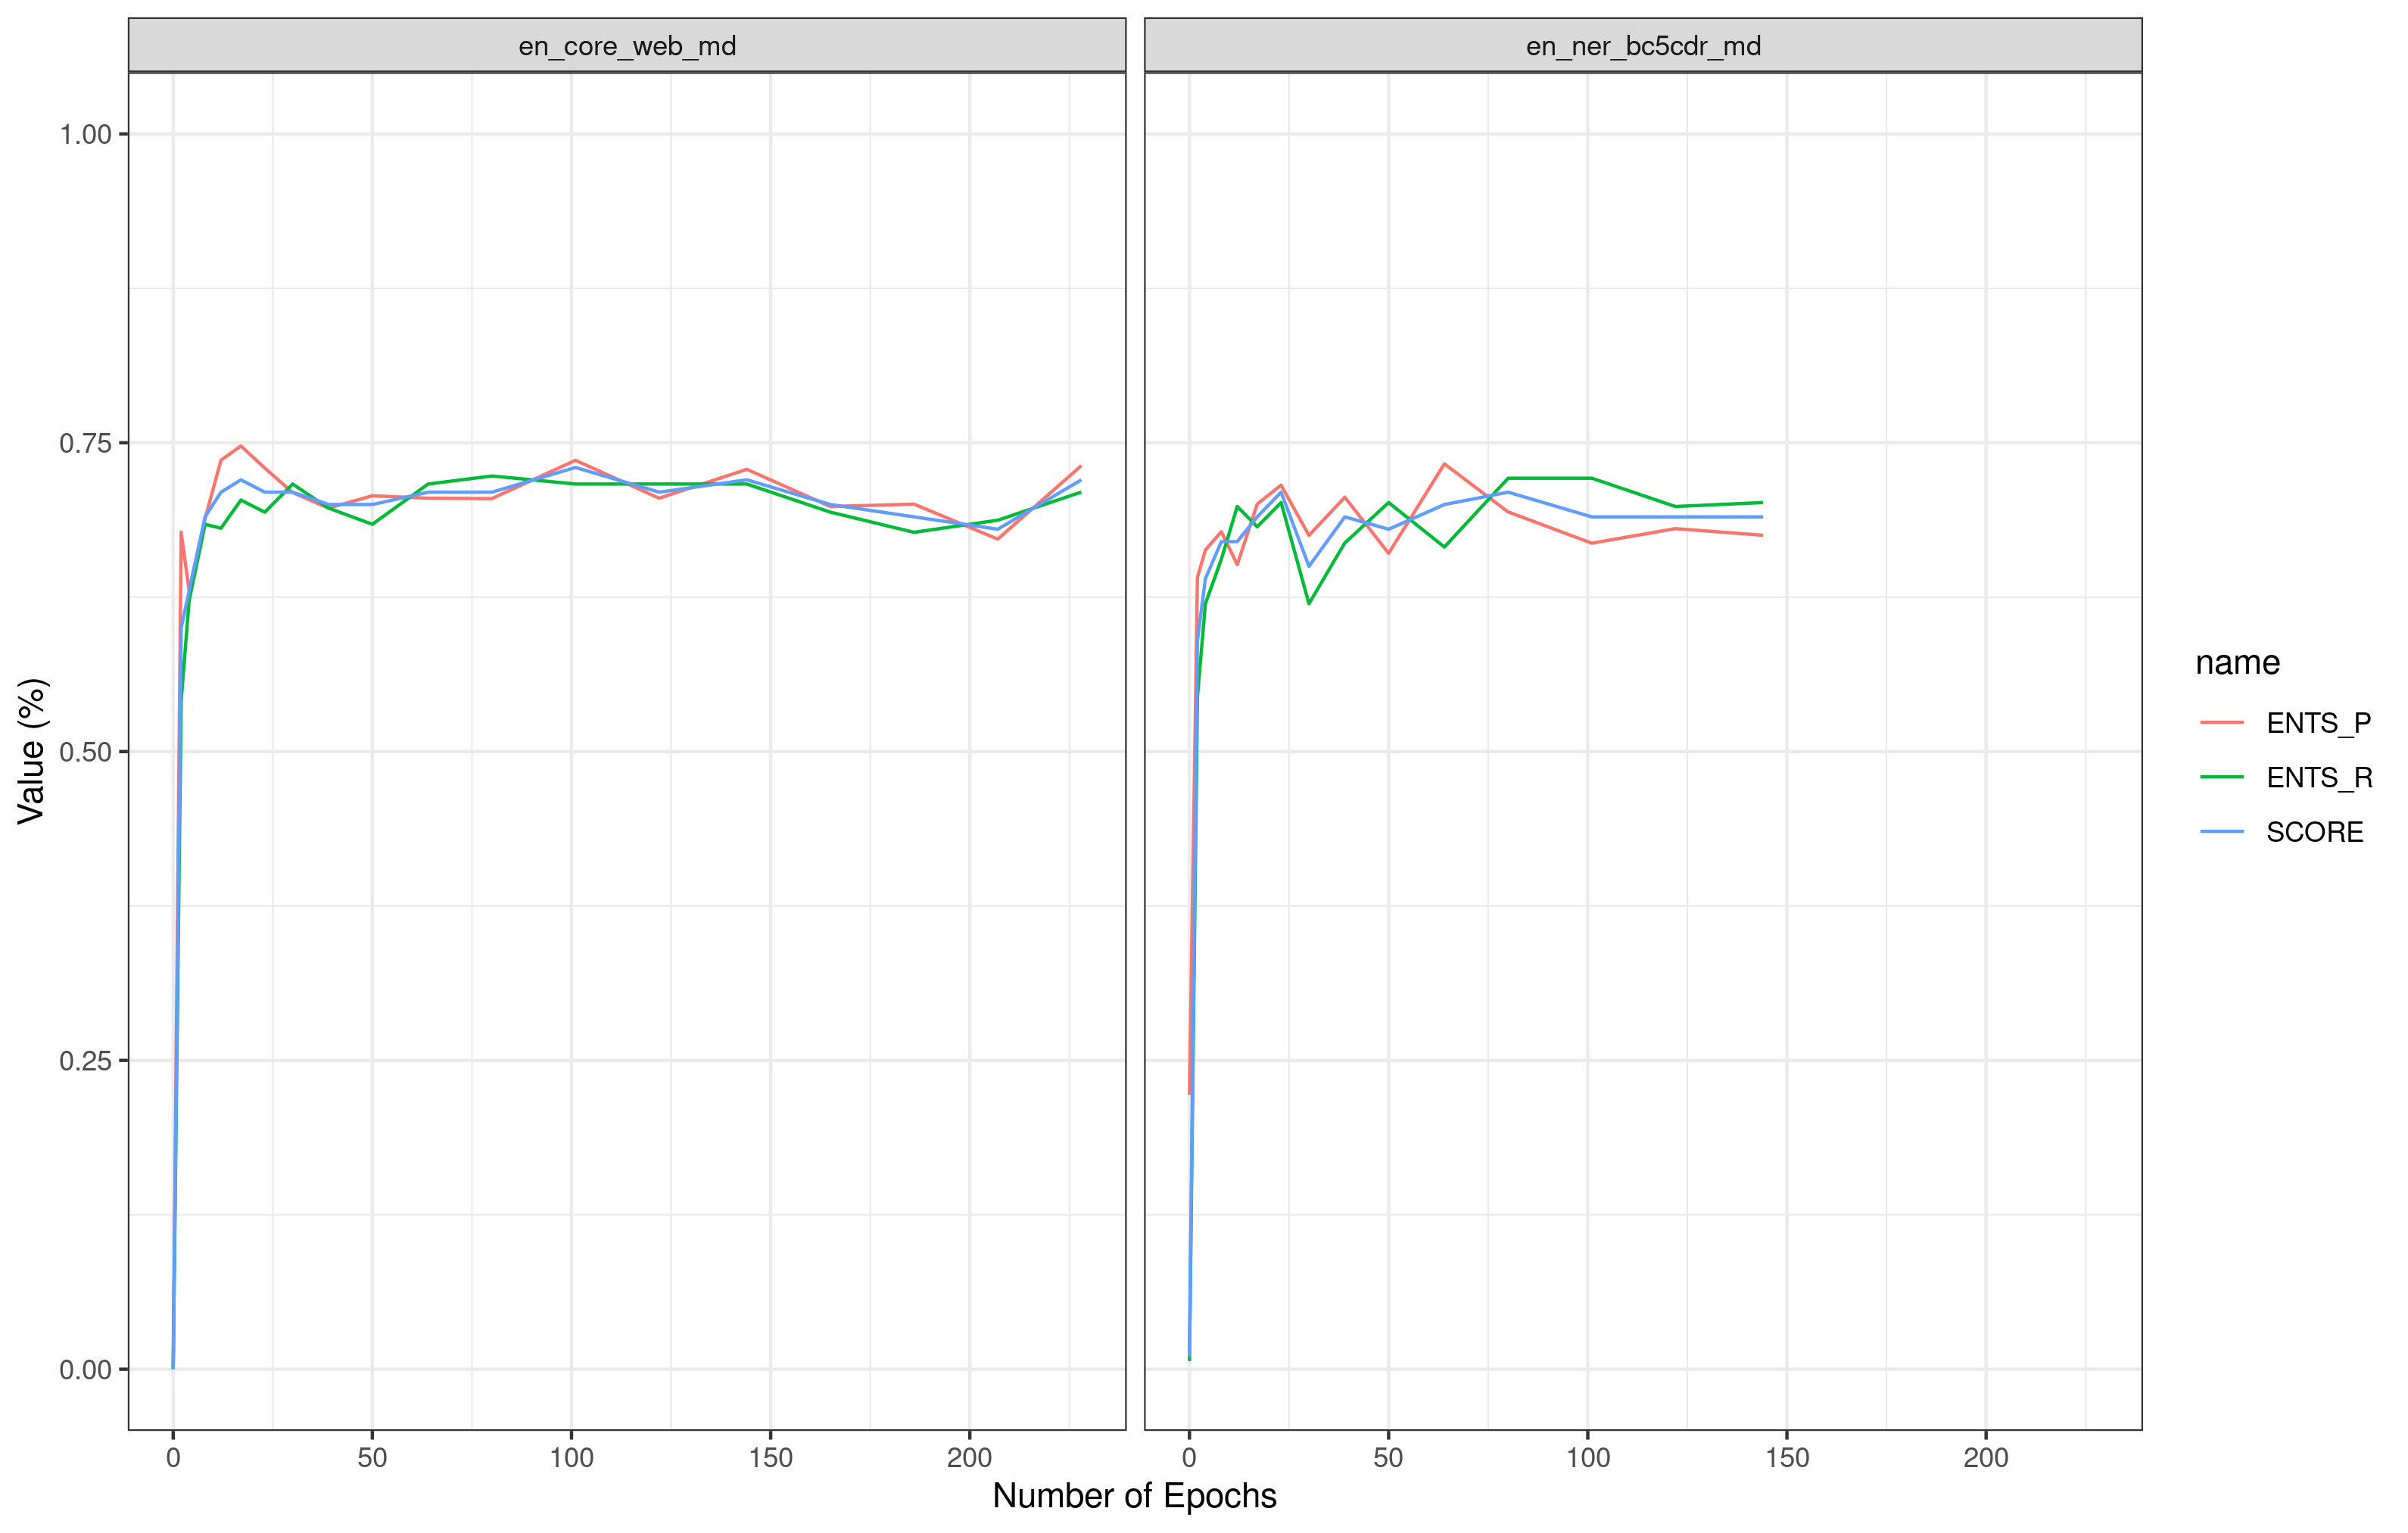
\includegraphics[width=1\textwidth]{spacy_train_precision_recall}
\end{figure}
In Abbildung \ref{fig:TrainPrecisionRecall} sind Precision, Recall und der f-Score des Trainings für zwei Basismodelle dargestellt. Diese sind das spaCy-eigene \glqq{en\_core\_web\_md}\grqq{} und das im Rahmen der BioCreative 5 Challenge erstellte \glqq{en\_ner\_bc5cdr\_md}\grqq. Für beide Modelle gilt, dass sich das Verhältnis von Precision und Recall über mehrere Trainingsepochen hinweg nicht wesentlich verbessert beziehungsweise stagnativ bei circa 70\% einpendelt. Die Wahl des Modells macht unter dieser Betrachtung folglich nicht wesentlich einen Unterschied. Dies deutet darauf hin, dass das Modell beim Training nicht wesentlich konvergiert, das heißt in XY übergeht.

Die Wahl des Basismodells für das weitere Annotieren sowie nachfolgende Schritte fiel dennoch auf das scispacy Modell, da dieses insgesamt mit mehr Daten trainiert wurde. Daher gehen wir davon aus, dass dieses Modell besser generalisieren wird, das heißt bei unbekannten Daten bessere Klassifikationen treffen wird.
% \footcite[vgl.]{zotero-163}\footcite[vgl.]{zotero-165}
\begin{figure}[H]
    \centering
    \caption[]{Verluste (\textit{losses}) bei \ac{NER} und TOK2VEC}
	\label{fig:TrainLosses}
    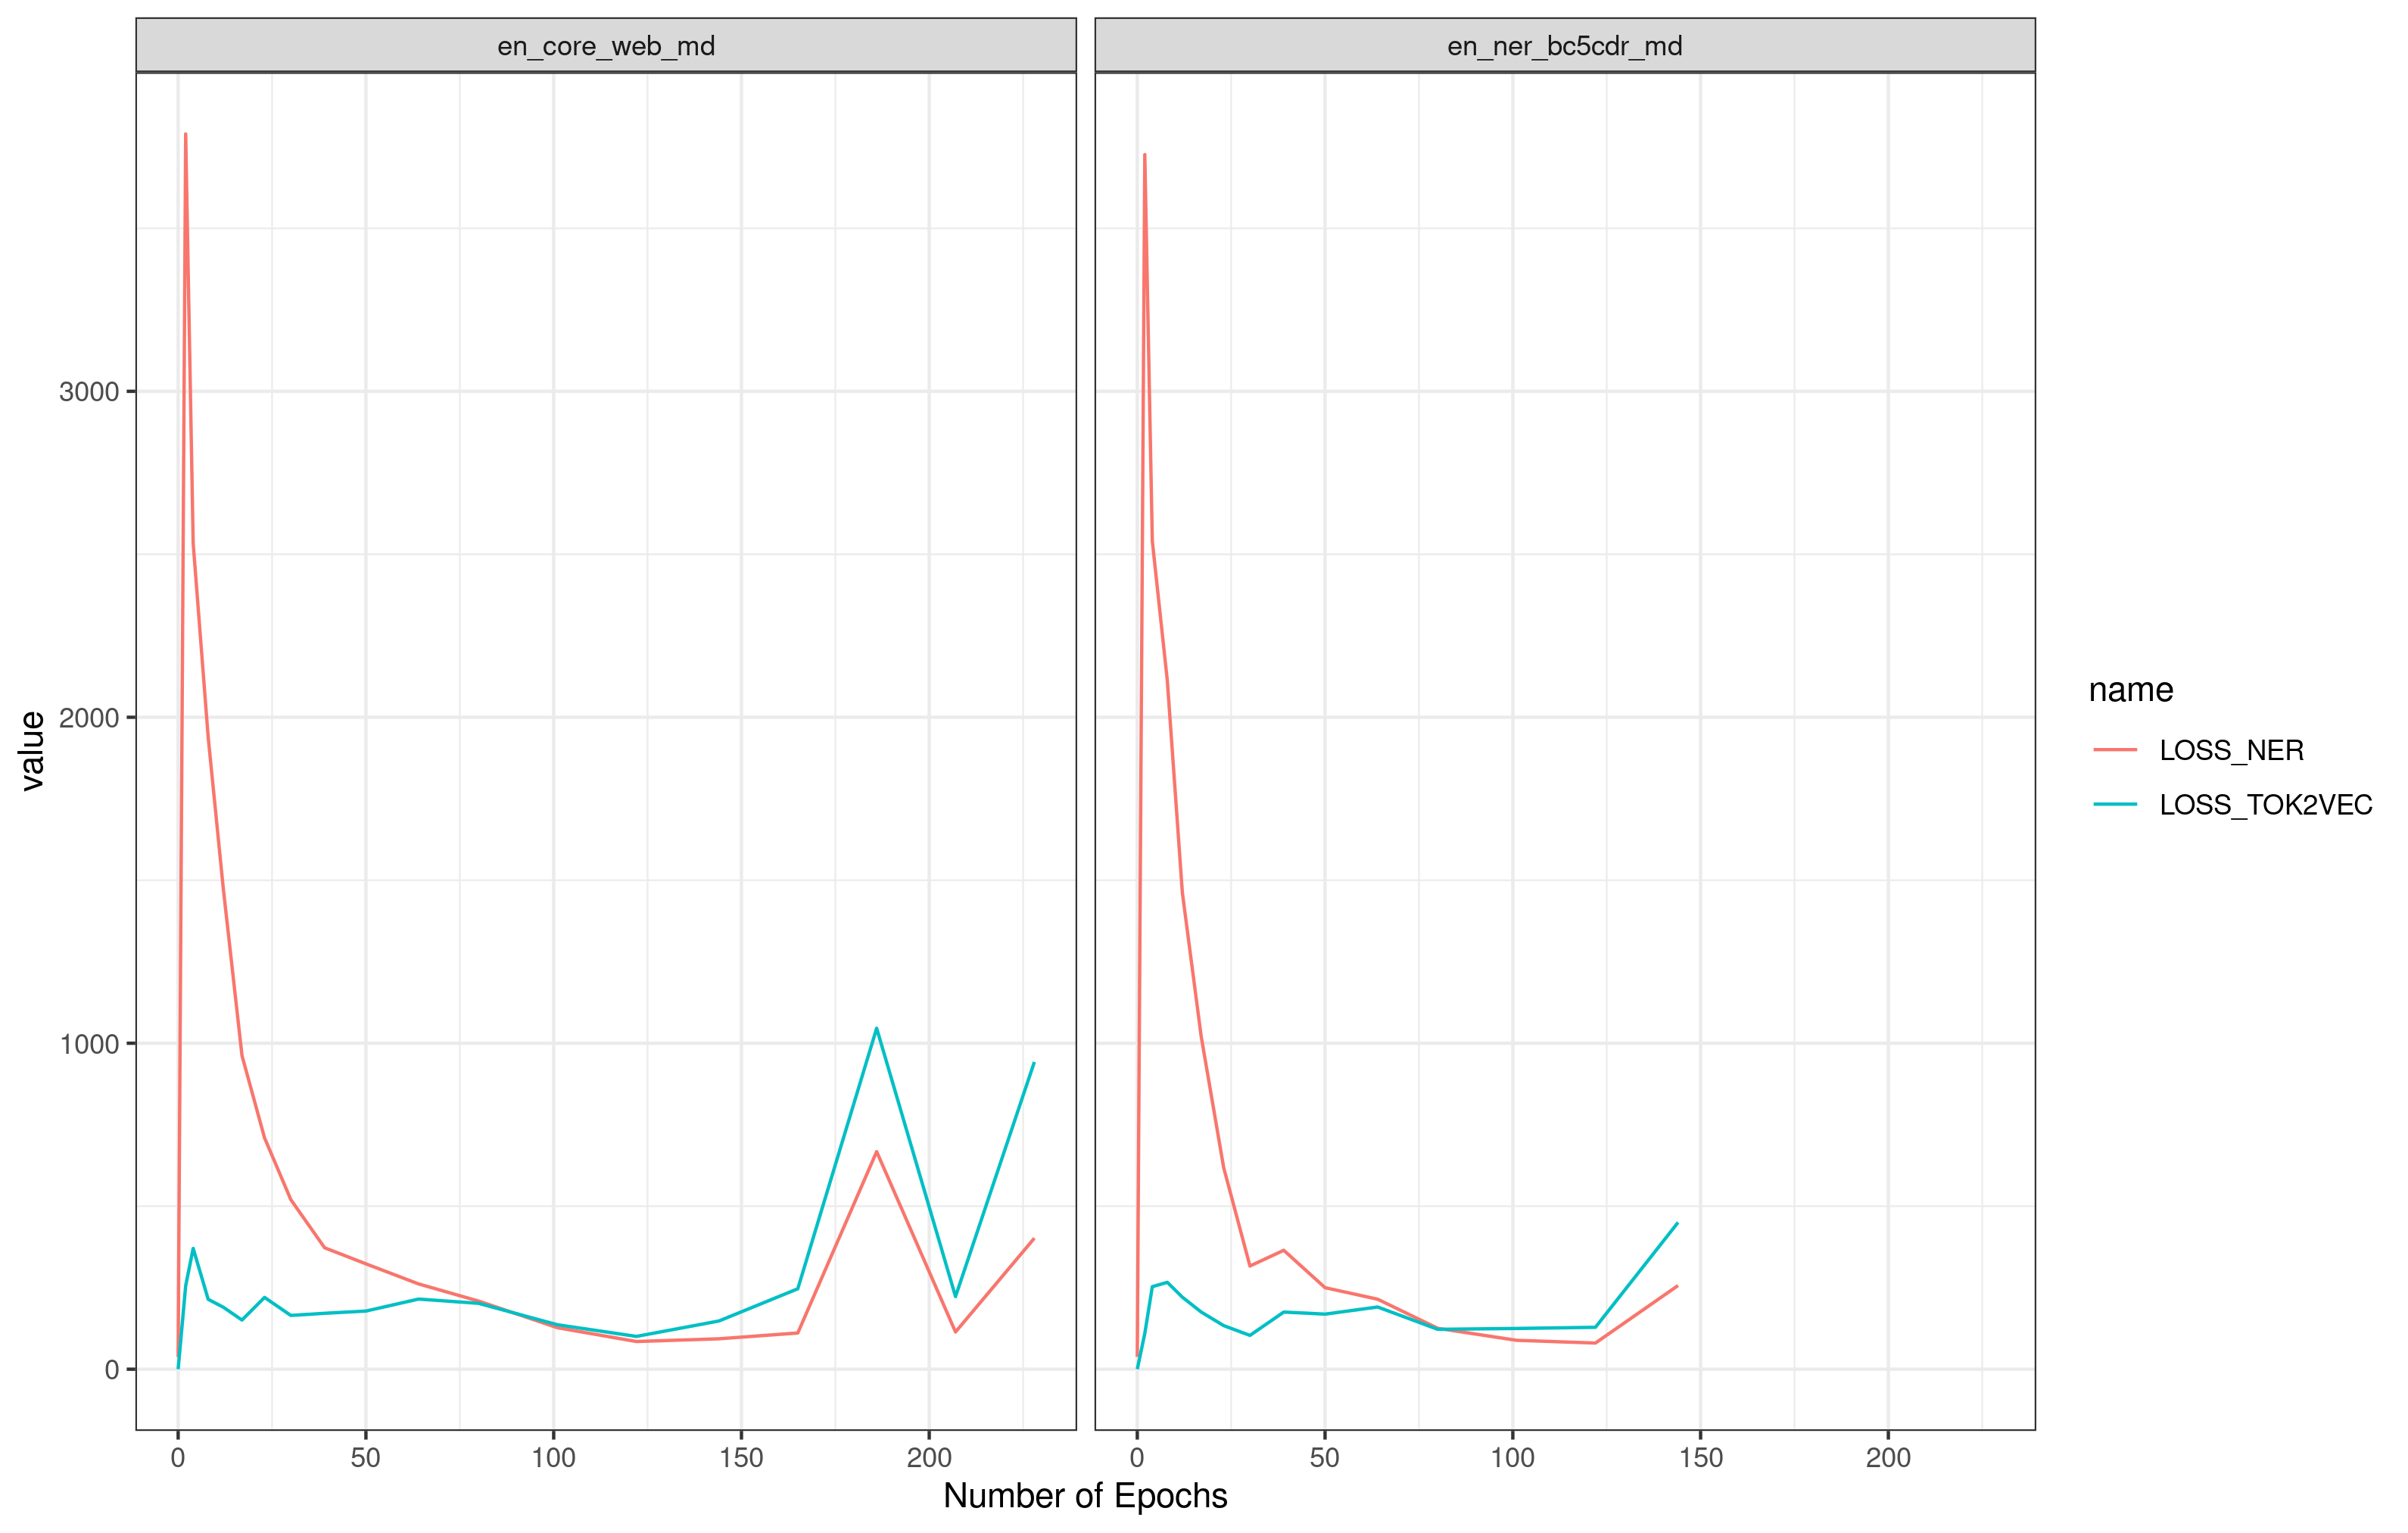
\includegraphics[width=1\textwidth]{spacy_train_losses}
\end{figure}
\footcite[]{tsai2006}

Was sind Verluste??

Zum weiteren Verständnis des Modells und der Vorhersagen, ist es sinnvoll, dieses feiner zu analysieren. So kann die Genauigkeit des Modells weiter für jede Entität aufgeschlüsselt werden.

\begin{figure}[H]
    \centering
    \caption[]{F-Score je Entität}
	\label{fig:TrainEntities}
    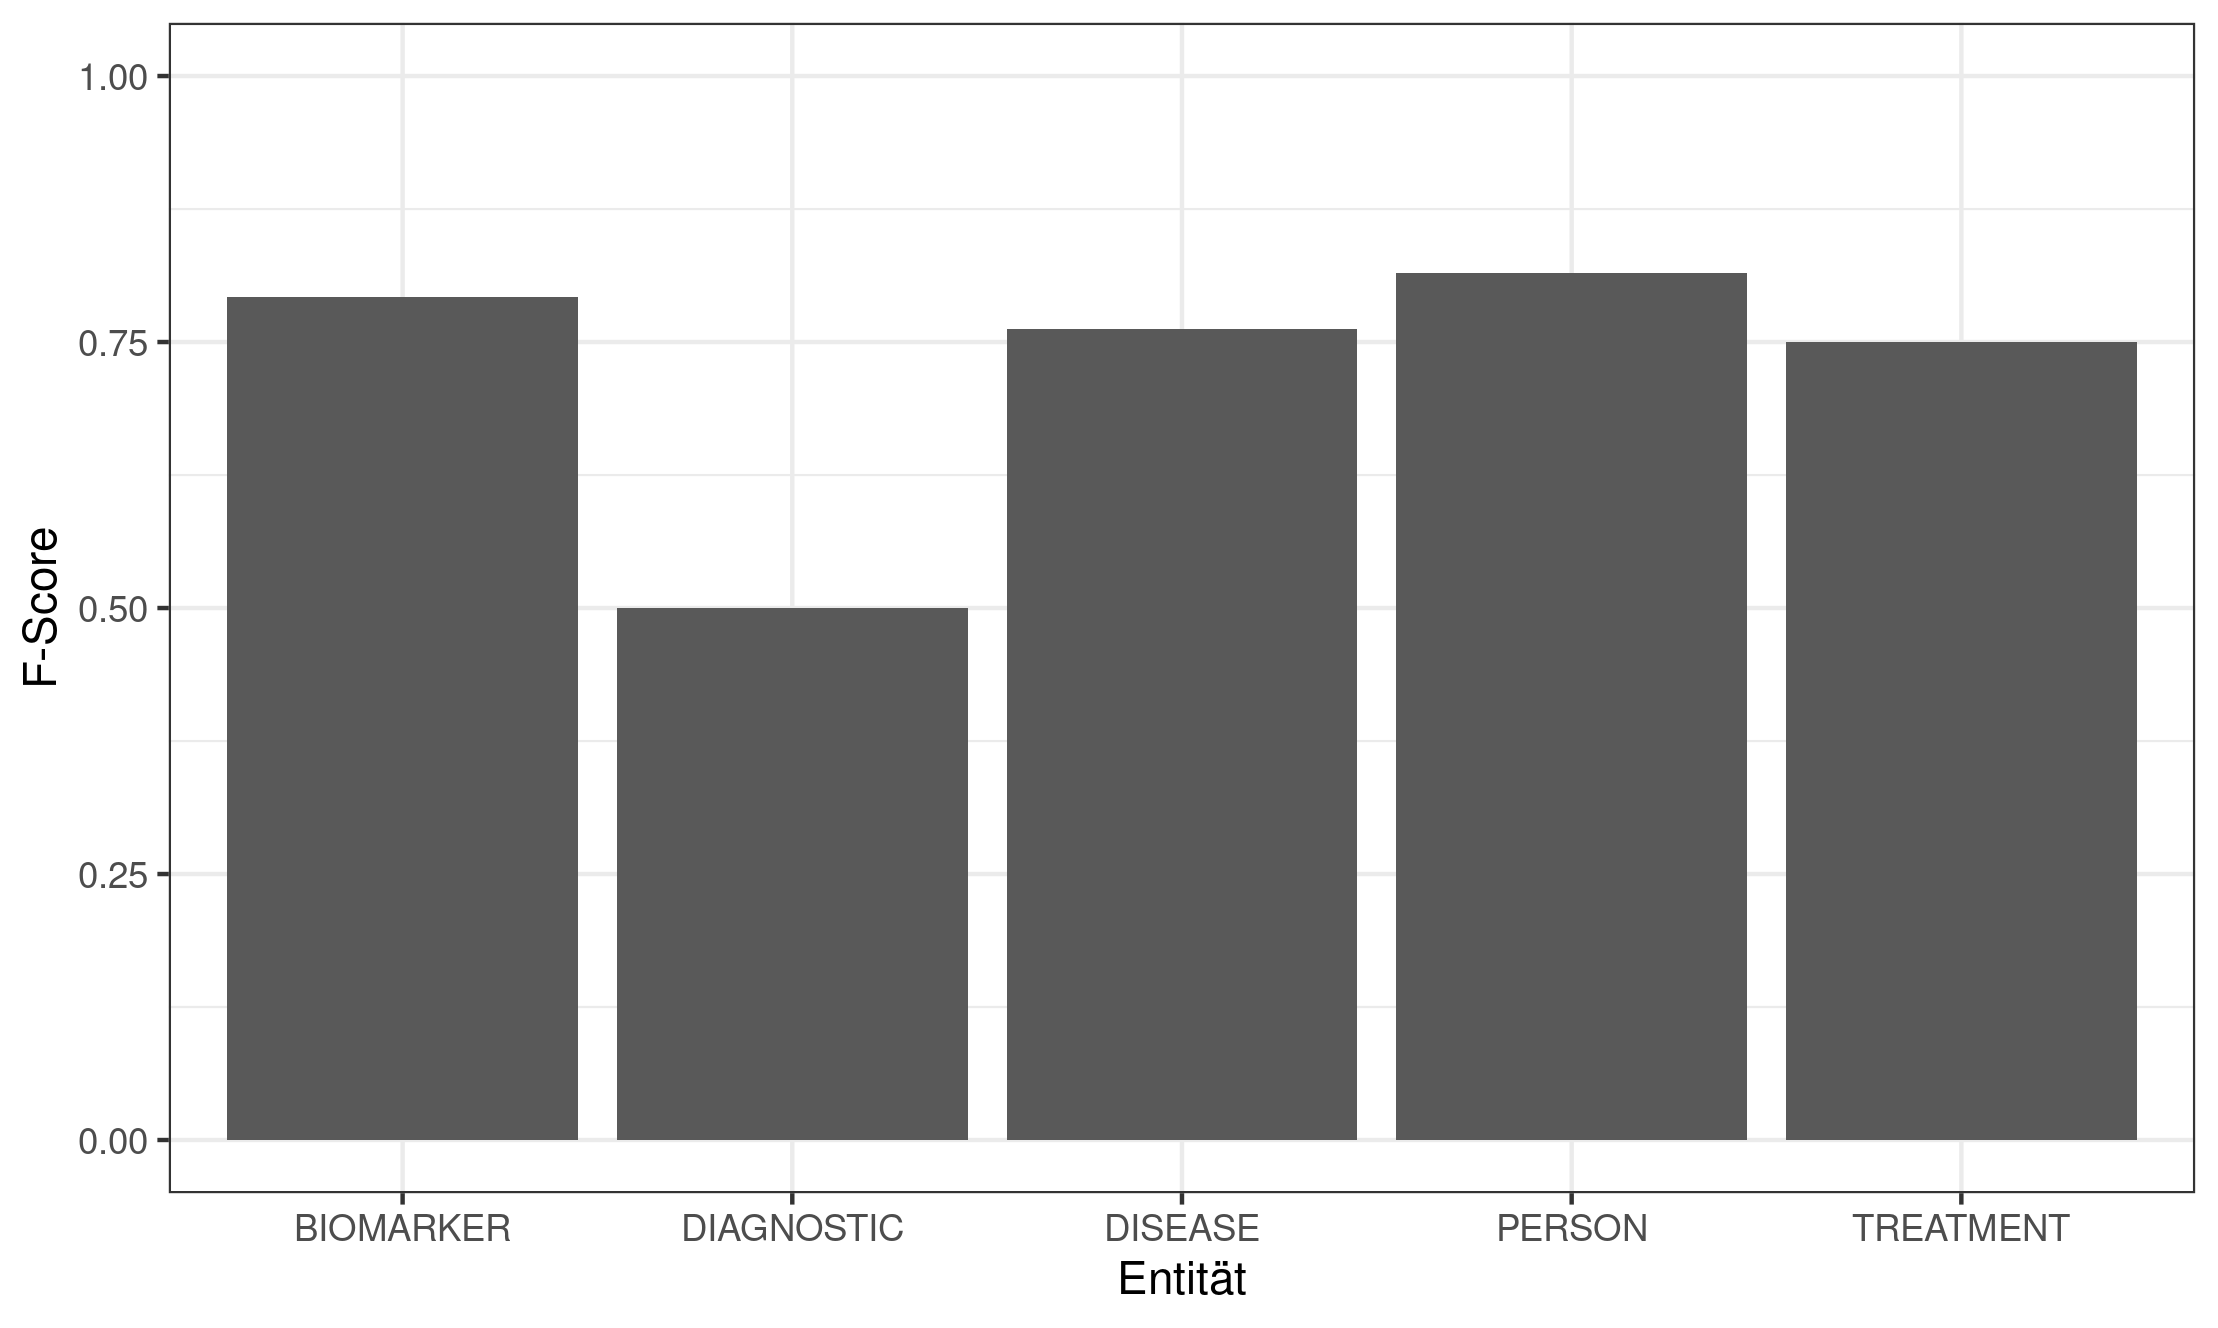
\includegraphics[width=1\textwidth]{spacy_train_entities}
\end{figure}
Abbildung \ref{fig:TrainEntities} stellt den F-Score je Entität dar. Es ist erkennbar, dass die Entitäten Biomarker, Disease, Person und Treatment einen sehr homogenen Score haben, Diagnostic jedoch deutlich darunter liegt. Ursächlich hierfür könnte die relativ geringe Anzahl an Trainingsdaten für das Diagnostic Label sein. Insgesamt liegt die Anzahl bei X, währenddessen bei den anderen Labels jeweils mindestens Y Textsamples vorhanden sind. Zur weiteren Verbesserung des F-Scores und somit des Modells, sollten folglich mehr Annotationen mit dem Diagnostic Label gesammelt werden.

% \subsection{Markeranalyse}
% \subsection{Überführung in Tabellenstruktur}
% \subsection{Markerkorrelationen}
% \subsection{Aufstellung des Gradingsystems}

\newpage
\section{Schlussbetrachtung}
(Umfang ca. 0,5 - 1 Seite)

\subsection{Zusammenfassung}

\subsection{Fazit}

\subsection{Kritische Reflexion}

\subsection{Ausblick}


%-----------------------------------
% Literaturverzeichnis
%-----------------------------------
\newpage
%\addcontentsline{toc}{section}{Literatur}

\pagenumbering{Roman} %Zähler wieder römisch ausgeben
\setcounter{page}{4}  %Zähler manuell hochsetzen

\printbibliography

% Alternative Darstellung:
% Literaturverzeichnis nach Typ (@book, @arcticle ...) sortiert.
% Dazu die Zeile (\printbibliography) auskommentieren und folgenden code verwenden:

%\printbibheading
%\printbibliography[type=article,heading=subbibliography,title={Artikel}]
%\printbibliography[type=book,heading=subbibliography,title={Bücher}]
%\printbibliography[type=online,heading=subbibliography,title={Webseiten}]

\newpage
\pagenumbering{gobble} % Keine Seitenzahlen mehr

%-----------------------------------
% Ehrenwörtliche Erklärung
%-----------------------------------
\section*{Ehrenwörtliche Erklärung}
Hiermit versichere ich, dass die vorliegende Arbeit von mir selbstständig und ohne unerlaubte Hilfe angefertigt worden ist, insbesondere dass ich alle Stellen, die wörtlich oder annähernd wörtlich aus Veröffentlichungen entnommen sind, durch Zitate als solche gekennzeichnet habe. Ich versichere auch, dass die von mir eingereichte schriftliche Version mit der digitalen Version übereinstimmt. Weiterhin erkläre ich, dass die Arbeit in gleicher oder ähnlicher Form noch keiner Prüfungsbehörde/Prüfungsstelle vorgelegen hat. Ich erkläre mich damit \textcolor{red}{einverstanden/nicht} einverstanden, dass die Arbeit der Öffentlichkeit zugänglich gemacht wird. Ich erkläre mich damit einverstanden, dass die Digitalversion dieser Arbeit zwecks Plagiatsprüfung auf die Server externer Anbieter hoch geladen werden darf. Die Plagiatsprüfung stellt keine Zurverfügungstellung für die Öffentlichkeit dar.

\par\medskip
\par\medskip

\_\_\_\_\_\_\_\_\_\_\_\_\_\_\_\_\_\_\_\_\_\_\_\_ \hspace{1.5cm} \_\_\_\_\_\_\_\_\_\_\_\_\_\_\_\_\_\_\_\_\_\_\_\_ \\
(Ort, Datum)\hspace{4.5cm}
(Eigenhändige Unterschrift)

\end{document}
